% !TEX root = ../presentation.tex


\begin{frame}{Landing Trajectory - Attitude}
    \begin{itemize}
        \item Goal: transition from  orbit about Itokawa to vertical descent
        \item Attitude controlled to point camera at surface
            \begin{itemize}
                \item \( \vb{b}_1 \) - body axis points at surface
                \item \( \vb{b}_3 \) - orthogonal projection in \( \vb{e}_3, \vb{b}_1\) plane
            \end{itemize}
    \end{itemize}
    \begin{columns}
        \begin{column}{0.5\textwidth}
        \begin{align*}
            \vb{b}_{1d} &= - \frac{\vb{x}}{\norm{\vb{x}}} , \\
            \vb{b}_{3d} &= \frac{\vb{f}_3 - \parenth{\vb{f}_3 \cdot \vb{b}_{1d}} \vb{b}_{1d}}{\norm{\vb{f}_3 - \parenth{\vb{f}_3 \cdot \vb{b}_{1d}} \vb{b}_{1d}}}, \\
            \vb{b}_{2d} &= \vb{b}_{3d} \times \vb{b}_{1d} , \\
        R_d &= \begin{bmatrix} \vb{b}_{1d} & \vb{b}_{2d} & \vb{b}_{3d} \end{bmatrix} .
        \end{align*}
    \end{column}
    \begin{column}{0.5\textwidth}
        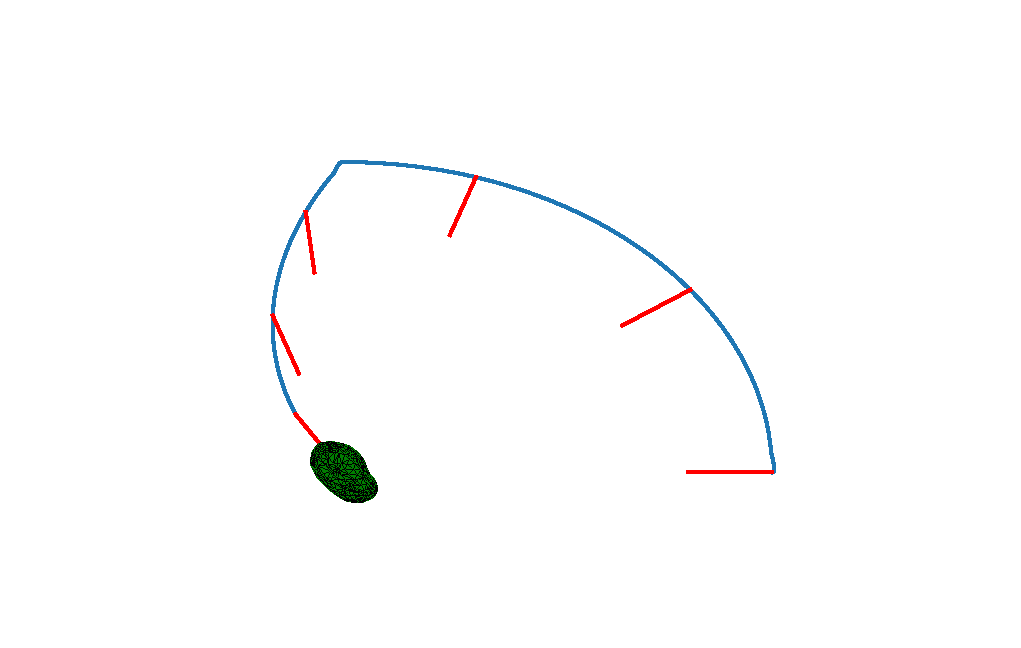
\includegraphics[width=\columnwidth,keepaspectratio,trim={30mm 20mm 30mm 20mm},clip]{figures/2017AAS_asteroid_landing/traj_fig.pdf}
\end{column}
\end{columns}
\end{frame}

\begin{frame}{Landing Trajectory - Position}
    \begin{itemize}
        \item Transition from horizontal motion to vertical descent
        \begin{itemize}
            \item Move from inertial \( \vb{e}_2 \) to asteroid \( \vb{f}_1 \) axis
            \item Remain in the equatorial plane ( \(\vb{f_1}, \vb{f}_2\) plane)
        \end{itemize}
        \pause
    \item Command is divided into two segments
        \begin{itemize}
            \item Move to \( \vb{f}_1\) along a circular path
            \item Vertical descent along \( \vb{f}_1 \)
        \end{itemize}
    \end{itemize}

    \begin{columns}
        \begin{column}{0.5\textwidth}
            \footnotesize
            \begin{align*}
                \vb{x}_d = 
                \begin{cases}
                    2.550 \begin{bmatrix} \sin{\omega t} & -\cos{\omega t} & 0 \end{bmatrix}, & t \leq t_d \\
                    R_A \begin{bmatrix} \frac{2}{t_d} (t - t_d) + 2.550 & 0 & 0 \end{bmatrix}, & t > t_d , 
                \end{cases}
            \end{align*}
        \end{column}
        \begin{column}{0.5\textwidth}
            \visible<2->{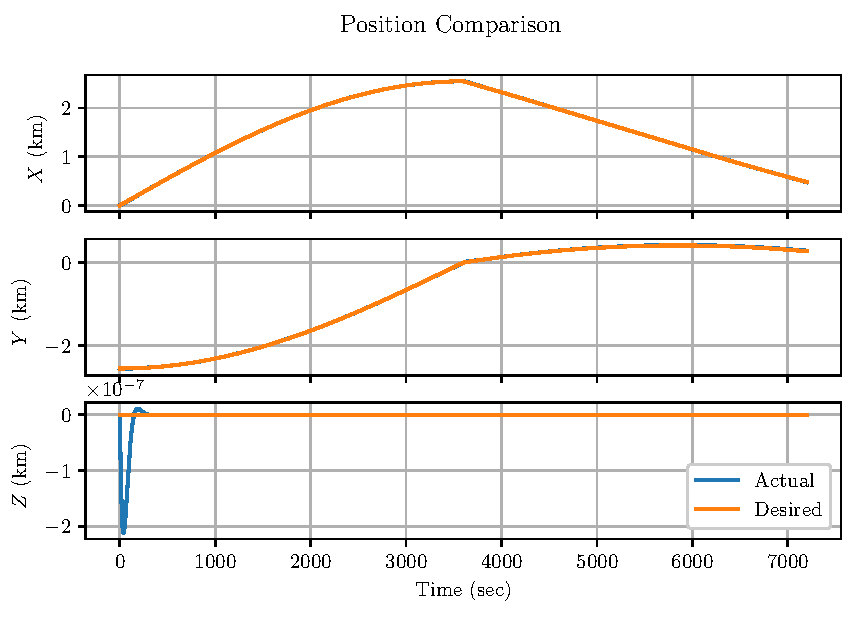
\includegraphics[width=\columnwidth]{figures/2017AAS_asteroid_landing/pos_fig.pdf}}
    \end{column}
\end{columns}
\end{frame}
